\documentclass[10pt]{article}

\usepackage[margin=0.78in]{geometry}
\usepackage[T1]{fontenc}
\usepackage{lmodern}
\usepackage{microtype}
\usepackage{amsmath,amssymb}
\usepackage{booktabs}
\usepackage{tabularx}
\usepackage{multirow}
\usepackage{enumitem}
\usepackage{xcolor}
\usepackage{graphicx}
\usepackage{caption}
\usepackage{subcaption}
\usepackage{tikz}
\usepackage{pgfplots}
\usepackage[numbers,sort&compress]{natbib}
\usepackage[hidelinks]{hyperref}
\usepackage{url}
\usepackage{fancyhdr}
\usepackage{xspace}

\usetikzlibrary{arrows.meta,positioning,fit,shapes.geometric}
\pgfplotsset{compat=1.18}
\setlist{nosep,leftmargin=*}
\setlength{\parskip}{0.35em}
\setlength{\parindent}{1em}
\captionsetup{font=small,labelfont=bf}
\urlstyle{same}

\definecolor{easiblue}{HTML}{275DAD}
\definecolor{easigreen}{HTML}{2A9D8F}
\definecolor{easired}{HTML}{C44536}
\definecolor{easigold}{HTML}{E9A23B}
\definecolor{easigray}{HTML}{5F6B7A}
\definecolor{easilight}{HTML}{F2F5F8}

\pagestyle{fancy}
\fancyhf{}
\lhead{EASI-Mem}
\rhead{Evidence-Aligned Safe Policy Evolution}
\cfoot{\thepage}
\renewcommand{\headrulewidth}{0.3pt}

\newcommand{\method}{\textsc{EASI-Mem}\xspace}
\newcommand{\base}{\textsc{Base}\xspace}
\newcommand{\rel}{\textsc{Relative-75}\xspace}
\newcommand{\code}[1]{\texttt{#1}}
\newcommand{\pp}{\,pp}

\title{\vspace{-1.2em}\textbf{EASI-Mem: Evidence-Aligned Safe Policy Evolution\\for Budgeted Long-Dialogue Memory}}
\author{Anonymous Authors}
\date{}

\begin{document}
\maketitle
\vspace{-1.2em}

\begin{abstract}
Long-horizon agents need memory policies that decide how many candidates to
retrieve and how much memory to inject, yet end-to-end task accuracy entangles
memory with the reader model, tools, prompting, and decoding. We present
\method, an evidence-aligned, bounded policy-evolution sidepath for the
open-source MemoryCore system. It preserves the existing FTS/vector substrate,
scores injected provenance units directly against public evidence annotations,
optimizes only a finite set of candidate and token-budget profiles, and promotes
a policy only when paired confidence and cost guards pass. Missing, corrupt,
incompatible, timed-out, or failed policies execute the exact base path.

On a 98-case LongMemEval-S held-out split, the development-selected policy
changes macro evidence-session recall from 82.40\% to 85.00\% while reducing
mean injected tokens by 30.09\%. The recall-delta 95\% interval is
$[-0.51,+6.07]$ percentage points, satisfying a predeclared 1-point
non-inferiority guard, and the joint utility interval is positive. We do not
present this as pristine confirmation because earlier protocol iterations had
exposed aggregate LongMemEval test results. More importantly, a
checksum-frozen transfer to 1,536 evidence questions in LoCoMo fails: tokens
fall 27.56\%, but macro session recall falls 4.52 points with a
conversation-cluster interval of $[-5.61,-3.35]$. An exploratory
leave-one-conversation-out calibration rejects every candidate and selects the
base path in 10/10 folds, preventing the harmful update but producing no gain.
These results establish a useful boundary: direct evidence feedback can support
cheap, auditable optimization and safe rejection, but a budget policy learned
on one dialogue distribution is not universally transferable. The release
includes dataset adapters, versioned protocols, structured receipts,
provenance persistence, a production switch, and forced-failure tests suitable
for later connection to internal multi-turn programming data.
\end{abstract}

\noindent\textbf{Keywords:} agent memory, long dialogue, self-optimization,
retrieval evaluation, provenance, safe fallback, token budget

\section{Introduction}

Persistent agents increasingly separate a bounded prompt from a larger memory
substrate. MemGPT frames this as virtual context management
\citep{packer2023memgpt}; systems such as Zep and Hindsight add temporal graphs,
typed memories, and reflection \citep{rasmussen2025zep,latimer2025hindsight}.
Open-source MemoryCore provides a layered substrate (raw L0 conversation, L1
atomic memory, L2 scenes, and L3 profiles), SQLite FTS5, vector search, fusion,
extraction, and injection \citep{memorycore2026}. In such systems, however,
\emph{policy} is commonly static: Top-$k$, candidate depth, and injection budget
are fixed at deployment.

Self-optimizing memory work makes this policy adaptive. Memory-R1 learns memory
operations through reinforcement learning \citep{yan2025memoryr1}; EvolveMem
searches an explicit configuration space with regression rollback
\citep{liu2026evolvemem}; and SelfMem lets an agent refine its memory strategy
from environmental feedback \citep{yang2026selfmem}. These approaches motivate
policy evolution, but they leave a practical systems question: how can an
existing memory service evolve a small, auditable policy without retraining or
replacing its retrieval core, and how can it refuse an update when the feedback
distribution shifts?

End-to-end answer accuracy is an expensive and noisy optimization target. A
failure may come from retrieval, reasoning, a tool, prompt construction, or
decoder variance. Conversely, a correct answer does not prove that injected
memory helped. LongMemEval and LoCoMo provide evidence annotations that permit
a more direct necessary-condition test: whether the memory boundary supplied
the labeled source units \citep{wu2024longmemeval,maharana2024locomo}.

We make four contributions:

\begin{enumerate}
  \item We define a provenance-aligned evaluation protocol that scores evidence
  sessions and turns separately from answer generation, together with exact
  injected-token and retrieval-latency costs.
  \item We introduce a bounded evolution layer over the unchanged MemoryCore
  retriever. A finite profile space, shallow confidence-gated router, versioned
  policy schema, and statistical promotion gate make adaptation reviewable.
  \item We implement a disabled-equivalent production sidepath with hard
  fallback and structured decision logs, plus L1 provenance persistence across
  SQLite and Tencent Cloud VectorDB paths.
  \item We report both positive developmental and negative external evidence.
  The latter reveals a granularity-induced transfer failure and demonstrates
  why safe rejection is part of optimization rather than an implementation
  afterthought.
\end{enumerate}

Our scope is deliberately narrow. Public long-dialogue data validates the
method; it does not establish performance on real long programming tasks.

\section{Related Work}

\paragraph{Agent memory systems.}
The field spans token-level, parametric, and latent forms, with factual,
experiential, and working-memory functions \citep{hu2025memorysurvey}.
MemGPT manages tiers around a finite context window \citep{packer2023memgpt}.
Zep's Graphiti component maintains a temporal knowledge graph
\citep{rasmussen2025zep}, while Hindsight separates facts, experiences,
observations, and beliefs and exposes retain/recall/reflect operations
\citep{latimer2025hindsight}. These systems improve memory representation and
lifecycle behavior. \method instead holds representation and the base
retriever fixed so that policy effects remain attributable.

\paragraph{Learned and evolving policies.}
Memory-R1 learns ADD, UPDATE, DELETE, and NOOP decisions and answer-side memory
selection \citep{yan2025memoryr1}. EvolveMem uses failure logs and a
meta-analyzer to modify retrieval configuration with revert-on-regression
\citep{liu2026evolvemem}. SelfMem exposes tools and feedback that permit broad
strategy refinement \citep{yang2026selfmem}. Our approach is less expressive:
it searches a pre-reviewed finite space and may emit only a bounded tree or
global leaf. The reduction in expressivity is intentional: it permits static
validation, exact fallback, and paired evaluation without model training.

\paragraph{Long-term memory evaluation.}
LongMemEval tests extraction, multi-session reasoning, temporal reasoning,
updates, and abstention over scalable chat histories
\citep{wu2024longmemeval}. LoCoMo supplies long multi-session conversations and
dialogue-level evidence annotations \citep{maharana2024locomo}. Their standard
QA evaluations measure useful end behavior, whereas our primary metric stops at
the injection boundary. This removes reader and judge variance but measures a
necessary, not sufficient, condition for correctness.

\paragraph{Retrieval infrastructure.}
MemoryCore's local substrate uses SQLite FTS5/BM25
\citep{sqlitefts5}; its broader hybrid path can combine rankings using reciprocal
rank fusion \citep{cormack2009rrf}. Our public experiment invokes the actual
MemoryCore L0 FTS5 path. We do not claim to improve BM25, FTS5, embeddings, or
RRF.

\section{Problem Formulation}

For query $q_i$, let $G_i^S$ and $G_i^T$ denote gold evidence sessions and
turns. A base retriever returns ordered candidates $C_i^{(K)}$ up to candidate
limit $K$. A policy $\theta$ selects a result limit $k$, token budget $B$, and
bounded reranking weights, producing injected units $I_i(\theta)$.

Our primary effectiveness statistic is macro evidence-session recall:
\begin{equation}
  R_S(\theta) = \frac{1}{N}\sum_{i=1}^{N}
  \frac{|S(I_i(\theta)) \cap G_i^S|}{|G_i^S|},
\end{equation}
where $S(I)$ extracts provenance session identifiers. We analogously compute
turn recall, any/all recall, and session NDCG \citep{jarvelin2002ndcg}. Cost is
the exact \code{cl100k\_base} token count $T_i(\theta)$ plus observed backend
query latency.

For comparison policy $a$ and base $b$, per-case utility is
\begin{equation}
 u_i(a,b) = R_{S,i}(a)-R_{S,i}(b)
 + \lambda\frac{T_i(b)-T_i(a)}{\overline{T(b)}},
 \qquad \lambda=0.03.
\end{equation}
The small cost coefficient cannot compensate for a large recall loss; recall
also has independent guards. A candidate is promoted only if:

\begin{align}
  \mathrm{LCB}_{.95}(\Delta R_S) &\ge -0.01, \\
  \Delta R_{\mathrm{any}},\Delta R_{\mathrm{all}} &\ge -0.01, \\
  1-\overline{T(a)}/\overline{T(b)} &\ge 0.10, \\
  \mathrm{UCB}_{.95}(\Delta T) &< 0, \\
  \mathrm{LCB}_{.95}(\Delta u) &> 0.
\end{align}

The evolution boundary is candidate/injection policy only. Storage semantics,
FTS5/vector kernels, and the extraction model are outside the action space.

\section{Method}

\subsection{Evidence-Aligned Adapter}

Every dataset adapter emits the same case object: stable case and dependency
group IDs; a query; ordered user/assistant turns with stable turn and session
IDs; gold turn/session sets; category; and a negative-load flag. The runtime
policy cannot receive answer, category, split, or gold labels.

LongMemEval's \code{has\_answer} turns define $G_i^T$, and
\code{answer\_session\_ids} define $G_i^S$. LoCoMo dialogue IDs in
\code{evidence} are mapped to their containing sessions. We append the
dataset-provided image caption and image-search query to image-bearing LoCoMo
turns, because some annotated facts are otherwise absent from text. Category-5
adversarial questions and four questions without evidence are negative-load
probes, not positive recall cases.

\subsection{Real MemoryCore Backend}

For every case, all turns are inserted through MemoryCore's SQLite-backed L0
schema. The runner calls the real \code{executeConversationSearch} function and
FTS5 index. Candidate IDs are original turn IDs; session IDs and timestamps are
preserved. This avoids a mock retriever that could accidentally encode labels.

We use L0 to isolate retrieval and injection. Evaluating L1 simultaneously
would add extraction-model and asynchronous-pipeline variance. To make later L1
evaluation possible, the implementation persists source-message provenance
through SQLite migrations/upserts/reads/FTS hydration, Tencent Cloud VectorDB,
and memory-search responses.

\subsection{Bounded Profile Space}

The v1.4 space contains eight profiles. \base returns Top-5 with no adaptive
token cap. \code{fixed-896} requests 30 candidates, returns at most 10, and caps
injection at 896 tokens. Six relative profiles use candidate limit 30, result
limit 10, and ratio $r \in \{.70,.75,.80,.85,.90,.95\}$:
\begin{equation}
  B_i(r) = \min\left(1024,\left\lfloor r T_i(\base)\right\rfloor\right).
\end{equation}
A greedy packer skips candidates that do not fit. Before packing, lexical
near-duplicate similarity may reduce a candidate's score by at most 12\%; a
recency multiplier is structurally capped at 10\%. The promoted v1.4 profiles
use no recency modulation.

The policy validator allows at most eight profiles, candidate limit 50, result
limit 12, budget 4,096, ratio $[.1,1]$, diversity weight .25, recency weight .10,
and router depth five.

\subsection{Evolution and Promotion}

Training cases receive a label from the best profile under a lexicographic
quality order (all-session recall, macro recall, any-session recall, NDCG, then
tokens). A shallow decision tree can split on query length/cues, corpus size,
and bounded Top-5 score, source-diversity, and token statistics. A leaf whose
majority confidence is below a configured threshold selects the globally safe
fallback. Global-profile and contextual-router promotion are evaluated
separately. Across v1.2--v1.4, contextual routers were rejected; v1.4 therefore
emits a static \rel{} leaf. The controller detects that no scout features are
needed and performs only one Top-30 query.

\begin{figure}[t]
\centering
\resizebox{0.98\textwidth}{!}{%
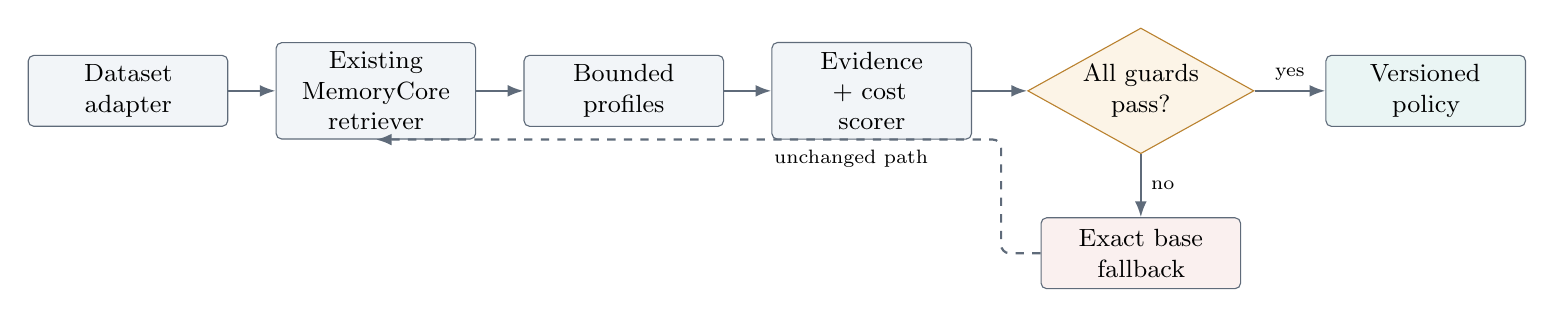
\begin{tikzpicture}[
  node distance=5mm and 6mm,
  box/.style={draw=easigray, rounded corners=2pt, fill=easilight, align=center,
    minimum height=9mm, text width=23mm, font=\small},
  gate/.style={diamond, draw=easigold!80!black, fill=easigold!12, align=center,
    aspect=1.8, inner sep=1pt, font=\small},
  arrow/.style={-{Latex[length=2mm]}, thick, draw=easigray}
]
\node[box] (adapter) {Dataset\\adapter};
\node[box, right=of adapter] (base) {Existing\\MemoryCore retriever};
\node[box, right=of base] (profiles) {Bounded\\profiles};
\node[box, right=of profiles] (score) {Evidence + cost\\scorer};
\node[gate, right=7mm of score] (gate) {All guards\\pass?};
\node[box, right=9mm of gate, fill=easigreen!10] (policy) {Versioned\\policy};
\node[box, below=8mm of gate, fill=easired!8] (fallback) {Exact base\\fallback};
\draw[arrow] (adapter) -- (base);
\draw[arrow] (base) -- (profiles);
\draw[arrow] (profiles) -- (score);
\draw[arrow] (score) -- (gate);
\draw[arrow] (gate) -- node[above,font=\scriptsize] {yes} (policy);
\draw[arrow] (gate) -- node[right,font=\scriptsize] {no} (fallback);
\draw[arrow, dashed, rounded corners=3pt]
  (fallback.west) -- ++(-5mm,0) |- node[pos=0.62,below,font=\scriptsize]
  {unchanged path} (base.south);
\end{tikzpicture}
}
\caption{The evolution loop changes only reviewed policy objects. The base
retriever remains available and is the terminal path for rejection or runtime
failure.}
\label{fig:architecture}
\end{figure}

\subsection{Production Execution and Fallback}

The production option is nested under \code{recall.adaptive} and defaults to
off. When off, auto-recall invokes the pre-existing search function directly.
When on, a read-only loader validates the versioned policy and verifies that
the runtime base profile matches the policy's evaluated baseline. The existing
retriever supplies candidates; the sidepath reranks and packs them; existing
character budgets remain an additional guard.

The decision log records mode, policy revision, profile, candidate and result
limits, effective token budget, returned items/tokens, fallback flag/reason,
and latency. A missing or malformed file, invalid schema/limit, baseline
mismatch, timeout, scout failure, or candidate-stage failure calls the exact
base query. The implementation does not delete or permanently replace an
index. A timed-out underlying call cannot be canceled if that retriever exposes
no abort interface, but its result is never injected.

\section{Experimental Protocol}

\subsection{Data and Splits}

Table~\ref{tab:data} gives immutable identifiers. LongMemEval-S-cleaned has 500
cases; 30 abstention cases are separated. Category-stratified hash ordering
with seed 20260823 assigns 280/92/98 retrieval cases to train/development/test.
All profiles share identical cases. Earlier protocol iterations inspected
aggregate test results, so the v1.4 test split is held out from v1.4 selection
but not pristine across the research process.

The LoCoMo file has 1,986 questions nested in ten conversations: 1,536
category 1--4 questions with explicit evidence and 450 negative-load probes.
The v1.4 policy JSON was frozen with SHA-256 before any LoCoMo retrieval run.

\begin{table}[t]
\centering
\small
\caption{Public data receipts.}
\label{tab:data}
\begin{tabularx}{\textwidth}{@{}lXrr@{}}
\toprule
Dataset & Immutable identifier & Scored & Groups \\
\midrule
LongMemEval-S-cleaned & HF rev. \code{98d7416c...d48f}; SHA-256
\code{d6f21ea9...3a442} & 470 & 470 cases \\
LoCoMo-10 & official file; SHA-256 \code{79fa87e9...98ff4} & 1,536 & 10 conversations \\
\bottomrule
\end{tabularx}
\end{table}

\subsection{Statistics and Cost}

We report means plus p50/p95 backend-query latency. LongMemEval comparisons use
5,000 paired bootstrap draws \citep{efron1993bootstrap}. Questions inside one
LoCoMo conversation are dependent, so its 5,000 draws resample whole
conversation clusters and then aggregate their paired cases. These intervals
represent sampling uncertainty under the public corpora, not systematic label
error.

The direct scorer makes no reader-model or LLM-judge calls. This is a central
cost advantage over repeated end-to-end trials, but we do not translate it into
dollars because hardware and provider pricing are deployment-specific.

\subsection{Protocol Evolution Audit}

Every change to split, metrics, or profile space increments the protocol and
reruns all baselines. Table~\ref{tab:history} retains negative iterations.

\begin{table}[t]
\centering
\small
\caption{Protocol history. ``Rejected'' means the candidate was not promoted.}
\label{tab:history}
\begin{tabularx}{\textwidth}{@{}llX@{}}
\toprule
Version & Outcome & Change and observation \\
\midrule
v1.0 & Rejected & Query-only contextual routing lost too much recall. \\
v1.1 & Rejected & Top-5 scout features did not recover utility confidence. \\
v1.2 & Safe/no gain & Conservative routing collapsed to the static fallback. \\
v1.3 & Global pass & Fixed 896-token profile passed LongMemEval; contextual routing failed; naive recency was harmful. \\
v1.4 & Mixed & Relative-budget policy passed development gates, then failed frozen LoCoMo transfer. \\
\bottomrule
\end{tabularx}
\end{table}

\section{Results}

\subsection{Developmental LongMemEval Result}

Development selection chooses \rel. On 98 held-out cases, macro session recall
rises from 0.82398 to 0.85000 and mean injected tokens fall from 1018.77 to
712.17. The recall delta is $+0.02602$ with paired 95\% interval
$[-0.00510,0.06071]$; token delta is $-306.59$
$[-346.28,-271.77]$; and utility is $+0.03505$
$[0.00431,0.07048]$. All promotion checks pass. The result supports method
development, not a final cross-domain claim.

\subsection{Frozen LoCoMo Transfer Failure}

The identical policy fails clearly on LoCoMo. Macro session recall changes from
0.74031 to 0.69516, a $-0.04516$ difference with cluster interval
$[-0.05612,-0.03354]$. Tokens fall from 168.71 to 122.20 (27.56\%), but utility
is negative: $-0.03689$ $[-0.04725,-0.02585]$. Any- and all-session recall also
fall by 4.88 and 4.10 points. The gate correctly rejects the transfer.

\begin{table}[t]
\centering
\small
\caption{Primary results. Recall is macro evidence-session recall. Confidence
intervals are paired for LongMemEval and conversation-clustered for LoCoMo.}
\label{tab:main-results}
\begin{tabular}{@{}lrrrrr@{}}
\toprule
Protocol & Base $R_S$ & Policy $R_S$ & $\Delta R_S$ 95\% CI & Base tok. & Policy tok. \\
\midrule
LongMemEval dev. & .8240 & .8500 & $[-.0051,.0607]$ & 1018.8 & 712.2 \\
LoCoMo frozen & .7403 & .6952 & $[-.0561,-.0335]$ & 168.7 & 122.2 \\
LoCoMo cross-fit & .7403 & .7403 & $[0,0]$ & 168.7 & 168.7 \\
\bottomrule
\end{tabular}
\end{table}

\begin{figure}[t]
\centering
\begin{subfigure}[t]{0.49\textwidth}
\centering
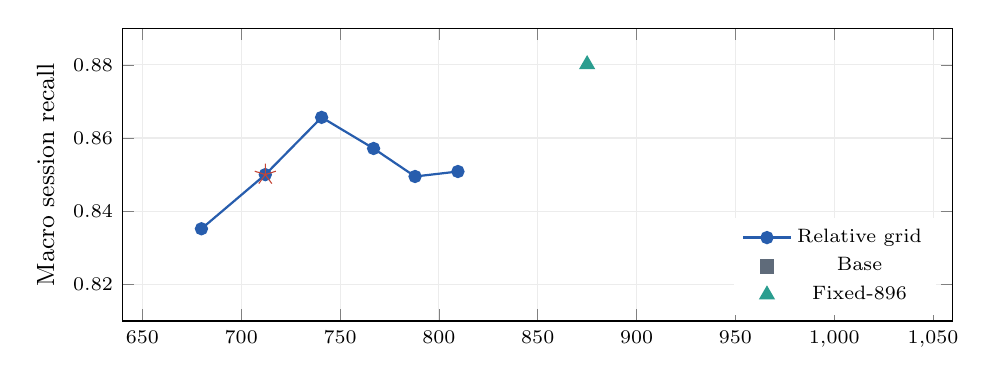
\begin{tikzpicture}
\begin{axis}[
  width=\linewidth,height=5.3cm,
  xlabel={},ylabel={Macro session recall},
  xmin=640,xmax=1060,ymin=.81,ymax=.89,
  grid=both,grid style={gray!15},
  tick label style={font=\scriptsize},label style={font=\small},
  legend style={font=\scriptsize,at={(0.98,0.02)},anchor=south east,draw=none,fill=white}
]
\addplot[color=easiblue,mark=*,thick] coordinates {
  (679.867,.835204) (712.173,.850000) (740.663,.865646)
  (766.949,.857143) (787.939,.849490) (809.622,.850850)
};
\addlegendentry{Relative grid}
\addplot[only marks,mark=square*,mark size=2.5pt,color=easigray] coordinates {(1018.765,.823980)};
\addlegendentry{Base}
\addplot[only marks,mark=triangle*,mark size=3pt,color=easigreen] coordinates {(874.980,.880102)};
\addlegendentry{Fixed-896}
\addplot[only marks,mark=star,mark size=4pt,color=easired] coordinates {(712.173,.850000)};
\end{axis}
\end{tikzpicture}
\caption{LongMemEval held-out.}
\end{subfigure}
\hfill
\begin{subfigure}[t]{0.49\textwidth}
\centering
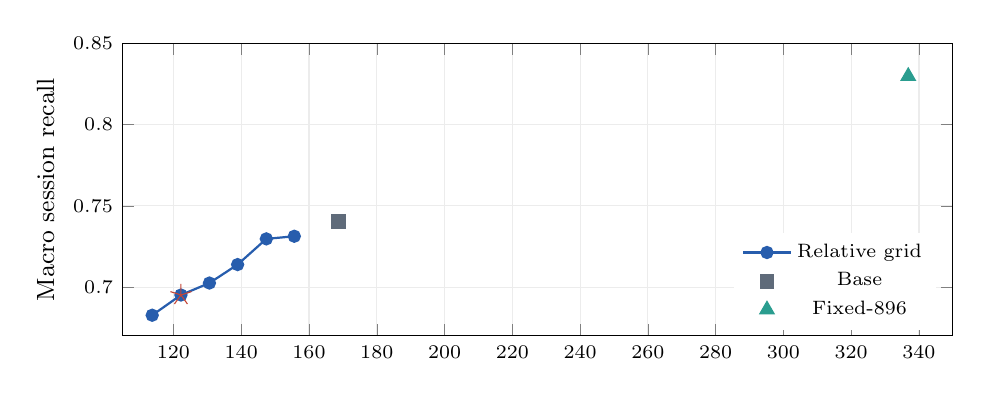
\begin{tikzpicture}
\begin{axis}[
  width=\linewidth,height=5.3cm,
  xlabel={},ylabel={Macro session recall},
  xmin=105,xmax=350,ymin=.67,ymax=.85,
  grid=both,grid style={gray!15},
  tick label style={font=\scriptsize},label style={font=\small},
  legend style={font=\scriptsize,at={(0.98,0.02)},anchor=south east,draw=none,fill=white}
]
\addplot[color=easiblue,mark=*,thick] coordinates {
  (113.725,.682725) (122.204,.695159) (130.613,.702517)
  (138.927,.713864) (147.400,.729662) (155.660,.731274)
};
\addlegendentry{Relative grid}
\addplot[only marks,mark=square*,mark size=2.5pt,color=easigray] coordinates {(168.708,.740314)};
\addlegendentry{Base}
\addplot[only marks,mark=triangle*,mark size=3pt,color=easigreen] coordinates {(336.833,.829664)};
\addlegendentry{Fixed-896}
\addplot[only marks,mark=star,mark size=4pt,color=easired] coordinates {(122.204,.695159)};
\end{axis}
\end{tikzpicture}
\caption{LoCoMo external stress test.}
\end{subfigure}
\caption{Macro evidence-session recall versus mean injected tokens. The policy
frontier is corpus-dependent. The red star is the
LongMemEval-selected \rel{} profile. It lies above-left of the LongMemEval base,
but below-left of the LoCoMo base.}
\label{fig:pareto}
\end{figure}

\subsection{Why Transfer Failed}

Figure~\ref{fig:pareto} shows a granularity shift rather than a random miss. A
base LongMemEval query contains 1018.8 tokens on average; a base LoCoMo query
contains only 168.7. Although the budget is relative, packing is discrete. At
75\%, the LoCoMo policy returns 4.21 items instead of the base five, frequently
removing an entire evidence turn. On LongMemEval it returns 6.38 shorter items
from a deeper pool, improving evidence coverage.

The fixed-896 control further clarifies the trade-off. On LoCoMo it improves
macro session recall to 0.82966 but doubles tokens to 336.83. No v1.4 arm
simultaneously satisfies the 1-point recall guard and 10\% token-saving gate.
Changing those thresholds after seeing the result would be protocol shopping,
so we retain the failure.

\subsection{Safe Rejection and Negative Load}

In exploratory leave-one-conversation-out calibration, each held-out
conversation selects a profile using the other nine. No candidate passes the
training-side guards in any fold; all 10/10 choose \base. The held-out result is
therefore byte-equivalent in policy behavior: no harm and no gain. The system
does not count rejection as optimization success.

The method does not solve abstention. On 30 LongMemEval abstention cases,
\rel{} injects 5.93 items versus 5.00 for base. On 450 LoCoMo negative-load
probes, it injects 4.19 items and 125.58 tokens versus 5.00 and 173.14 for base.
Reducing irrelevant load is useful, but a calibrated zero-injection decision
requires explicit sufficiency supervision.

\subsection{Latency}

LongMemEval backend query p50/p95 increases from 0.662/1.648 ms to
1.326/2.348 ms when the candidate limit grows from 5 to 30. LoCoMo increases
from 0.379/0.561 ms to 0.833/1.089 ms. These local in-memory measurements are
small in absolute terms but roughly double retrieval latency; remote vector
stores must be remeasured rather than extrapolated.

\section{Transfer to Long Programming Tasks}

The code separates dataset semantics from the optimizer. An internal adapter
would map a task/conversation to a dependency group, the current request to a
query, and immutable user messages, tool results, patches, commits, or test
failures to provenance units. Explicit ``you forgot'' feedback is precise but
sparse; accepted patches, repeated constraints, reversions, and controlled test
outcomes can provide weaker labels with confidence weights.

Three public-data assumptions will fail in programming sessions. First,
evidence may be an ordered causal chain rather than an unordered set. Second,
tool and repository state may be necessary even when no message contains the
answer. Third, later decisions can supersede earlier evidence. A programming
protocol should therefore add ordered-chain recall, state snapshot identifiers,
supersession labels, and a penalty for injecting stale or contradicted memory.
These changes belong in a versioned adapter/metric protocol; they do not require
rewriting the policy controller.

The recommended rollout is conservative: collect provenance and direct labels;
run base and candidate policies offline; require task-cluster confidence gates;
publish a signed/versioned policy; canary the sidepath; and retain immediate
base fallback. End-to-end coding-agent trials should follow, not replace, the
direct memory gate.

\section{Limitations and Threats to Validity}

\paragraph{Necessary, not sufficient.}
Evidence recall does not show that a reader used evidence correctly. It also
cannot certify that an arbitrary truncation preserves the answer-bearing span.
We therefore score intact provenance units and do not claim QA accuracy.

\paragraph{Development contamination.}
Protocol v1.4 followed three LongMemEval iterations whose aggregate test results
were inspected. Its confidence interval is statistically paired but does not
correct researcher adaptivity. We label it developmental and use the frozen
LoCoMo result to test transfer.

\paragraph{Dataset dependence.}
LoCoMo has 1,536 evidence questions but only ten independent conversations.
Cluster bootstrap respects this structure, yet ten clusters remain a small
external sample. LoCoMo annotations and provided image text may contain their
own errors.

\paragraph{Retriever scope.}
The public run evaluates L0 SQLite FTS5 only. It does not establish behavior for
L1 extraction, embeddings, hybrid RRF, TCVDB latency, or a real HTTP deployment.
The provenance and adapter work enables those experiments but does not substitute
for them.

\paragraph{Cost proxy.}
\code{cl100k\_base} is reproducible but may differ from a deployed model's
tokenizer. Latency excludes network and downstream generation. The 250 ms
sidepath timeout controls returned behavior but cannot cancel a retriever that
does not expose abort.

\paragraph{Programming claim boundary.}
Neither public corpus is a long programming benchmark. We demonstrate a
portable method and failure-safe implementation, not production coding-agent
improvement.

\section{Reproducibility, Artifacts, and Ethics}

The release records dataset revision/checksum, protocol JSON, split seed, all
profile definitions, 5,000 bootstrap draws, structured case outputs, compact
result receipts, and the promoted policy checksum. The implementation is on a
dedicated branch over MemoryCore v2 source. Unit tests cover disabled-path
equivalence, corrupt policy, baseline mismatch, forced adaptive error, timeout,
hard limits, base-relative budget, and L1 provenance round-trip. The complete
plugin build is also exercised.

No private user or programming data is used. LongMemEval and LoCoMo are public;
LoCoMo's CC BY-NC 4.0 terms must be respected. Direct evidence logs can expose
sensitive user text in a real deployment, so internal reports should store
stable source IDs and bounded diagnostics rather than raw content whenever
possible.

\section{Conclusion}

\method makes memory policy evolution measurable and reversible without
rewriting MemoryCore's retrieval substrate. On LongMemEval it finds a
developmentally useful recall/token trade-off. The same checksum-frozen policy
fails on LoCoMo, where shorter turns turn a token ratio into an item-deletion
policy. A leave-one-conversation-out gate rejects every candidate and returns
the exact base path. The honest conclusion is not that one Top-$k$ or token
ratio is universally optimal; it is that evidence-aligned feedback, bounded
search, versioned receipts, and the ability to reject evolution are all
necessary for trustworthy memory self-optimization. The next evaluation should
connect the same interfaces to provenance-rich long programming sessions and
add state, order, and supersession-aware evidence.

\bibliographystyle{plainnat}
\bibliography{references}

\appendix
\section{Runtime Configuration Example}

\begin{verbatim}
{
  "recall": {
    "maxResults": 5,
    "adaptive": {
      "enabled": true,
      "policyPath": "policies/easi-mem-v1.4.json",
      "timeoutMs": 250
    }
  }
}
\end{verbatim}

The feature defaults to disabled. A relative path is resolved below the plugin
data directory. The policy's declared base must match \code{maxResults}; a
mismatch is logged and falls back.

\section{Structured Decision Example}

\begin{verbatim}
{
  "mode": "adaptive",
  "policyRevision": "easi-adc30593739a",
  "selectedProfile": "relative-75",
  "candidateLimit": 30,
  "resultLimit": 10,
  "tokenBudget": 742,
  "returnedItems": 7,
  "returnedTokens": 718,
  "fallback": false,
  "latencyMs": 2.31
}
\end{verbatim}

Fallback decisions use \code{mode=base}, \code{fallback=true}, and a bounded
reason indicating policy validation or adaptive-stage failure. No error path
silently returns an empty adaptive set as if it were a valid optimization.

\end{document}
